\documentclass[12pt]{article}
\usepackage[utf8]{inputenc}
\usepackage[T1]{fontenc}
\usepackage{geometry}
\geometry{margin=1in}
\usepackage{hyperref}
\usepackage{tikz}
\usepackage{pgfplots}
\usepackage{algorithm}
\usepackage{algpseudocode}
\usepackage{amsmath}
\usepackage{amssymb}
\usepackage{graphicx}
\usepackage{listings}
\usepackage{xcolor}
\usepackage{float}
\usepackage{tabularx}
\usetikzlibrary{shapes,arrows,positioning,calc,backgrounds,fit}
\pgfplotsset{compat=1.18}
\title{Sistema Distribuido Master-Slave con Ubicación Semántica}
\author{Abel Ponce González C411\\Richard Alejandro Matos Arderí C411}
\date{\today}

\begin{document}

\maketitle

\begin{abstract}
Este documento presenta la especificación arquitectónica de un sistema distribuido de búsqueda de documentos basado en arquitectura Master-Slave con elección dinámica de líder. Se detalla la arquitectura del sistema, la organización y roles de sus componentes, los mecanismos de ubicación de recursos mediante vectorización semántica, las estrategias de tolerancia a fallos con algoritmo Bully para elección de líder, el sistema de replicación por afinidad semántica, y los aspectos de seguridad y comunicación del diseño.
\end{abstract}

\tableofcontents

\newpage

\section{Introducción}

\subsection{Descripción del sistema}
El sistema propuesto es una plataforma distribuida para almacenamiento y búsqueda de documentos utilizando una arquitectura Master-Slave con elección dinámica de líder. El sistema emplea vectorización semántica para ubicación de recursos, lo que permite localizar documentos basándose en similitud de contenido en lugar de funciones hash. Esta aproximación proporciona búsquedas más relevantes y una distribución de datos más inteligente basada en afinidad de contenido.

\subsection{Objetivos del diseño}
\begin{itemize}
  \item Proporcionar alta disponibilidad mediante elección automática de líder ante fallos del Master
  \item Garantizar redundancia de datos mediante replicación basada en afinidad semántica
  \item Proporcionar mecanismos eficientes de localización de recursos mediante vectorización semántica
  \item Implementar tolerancia a fallos con detección mediante heartbeats y recuperación automática
  \item Distribuir carga entre Slaves mediante balanceo basado en carga y afinidad de contenido
  \item Permitir acceso distribuido mediante DNS con múltiples puntos de entrada
\end{itemize}

\section{Arquitectura del Sistema}

\subsection{Estilo arquitectónico}

\subsubsection{Clasificación según estilos arquitectónicos}

El sistema sigue un \textbf{estilo arquitectónico Master-Slave} con capacidad de promoción dinámica. En este modelo, un nodo asume el rol de Master (coordinador) mientras los demás actúan como Slaves (trabajadores). La característica distintiva es que cualquier Slave puede convertirse en Master mediante un proceso de elección cuando el Master actual falla, eliminando así el punto único de fallo típico de arquitecturas centralizadas.

Los componentes principales son:
\begin{itemize}
  \item \textbf{Nodos Slave}: Unidades autónomas que almacenan documentos, procesan búsquedas locales y mantienen su propia instancia de MongoDB. Cada Slave incluye tanto backend (API FastAPI) como frontend (interfaz de usuario).
  \item \textbf{Master}: Un Slave que asume responsabilidades adicionales de coordinación: mantiene el índice de ubicación semántica global, balancea carga entre Slaves, coordina replicación y enruta queries distribuidas.
  \item \textbf{Sistema DNS}: Proporciona resolución de nombres con múltiples entradas para failover automático.
\end{itemize}

\subsection{Modelo arquitectónico: Master-Slave con elección dinámica}

\subsubsection{Características del sistema}

El sistema implementa una arquitectura \textbf{Master-Slave con failover automático}. A diferencia de arquitecturas centralizadas tradicionales, el rol de Master no está fijado a un nodo específico sino que puede migrar dinámicamente entre los Slaves candidatos cuando ocurre una falla.

\textbf{Ubicación de recursos por vectorización semántica:} En lugar de utilizar funciones hash para determinar dónde almacenar documentos (como en DHT), el sistema emplea embeddings semánticos generados mediante sentence-transformers. Cada documento se representa como un vector de 384 dimensiones que captura su significado semántico. El Master mantiene un índice de ubicación que mapea embeddings a los Slaves que contienen documentos similares, permitiendo:
\begin{itemize}
  \item Routing inteligente de queries a Slaves con contenido relevante
  \item Selección de nodos para replicación basada en afinidad de contenido
  \item Balanceo de carga considerando tanto capacidad como especialización de contenido
\end{itemize}

\begin{figure}[H]
\centering
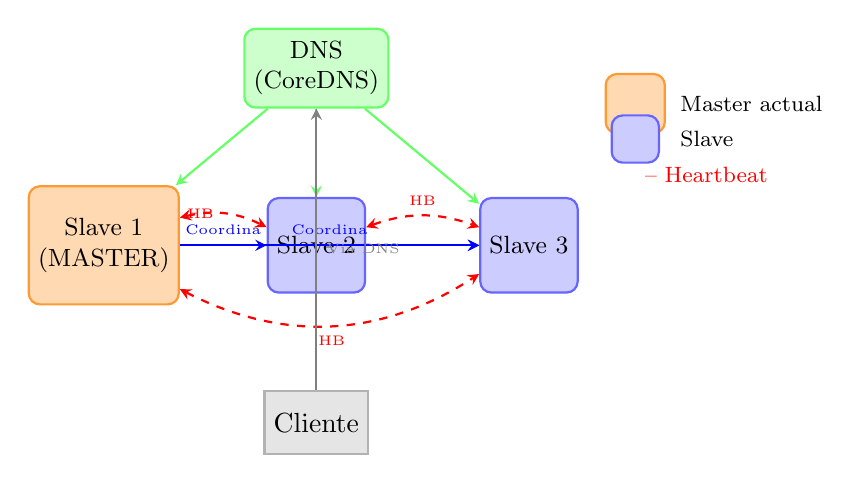
\begin{tikzpicture}[scale=0.9]
  % Definir estilos
  \tikzstyle{master}=[rectangle, draw=orange!80, fill=orange!30, thick, minimum size=1.5cm, font=\small, rounded corners, align=center]
  \tikzstyle{slave}=[rectangle, draw=blue!60, fill=blue!20, thick, minimum size=1.2cm, font=\small, rounded corners, align=center]
  \tikzstyle{dns}=[rectangle, draw=green!60, fill=green!20, thick, minimum size=1cm, font=\small, rounded corners, align=center]
  \tikzstyle{client}=[rectangle, draw=gray!60, fill=gray!20, thick, minimum size=0.8cm, align=center]
  \tikzstyle{conn}=[->, thick, >=stealth]
  \tikzstyle{heartbeat}=[<->, thick, >=stealth, red, dashed]
  
  % DNS
  \node[dns] (dns) at (3,5) {DNS \\ (CoreDNS)};
  
  % Master (actualmente Slave 1)
  \node[master] (master) at (0,2.5) {Slave 1 \\ (MASTER)};
  
  % Slaves
  \node[slave] (s2) at (3,2.5) {Slave 2};
  \node[slave] (s3) at (6,2.5) {Slave 3};
  
  % Cliente
  \node[client] (c1) at (3,0) {Cliente};
  
  % Conexiones Master-Slave
  \draw[conn, blue] (master) -- node[above, font=\tiny] {Coordina} (s2);
  \draw[conn, blue] (master) -- node[above, font=\tiny] {Coordina} (s3);
  \draw[conn, blue] (s2) -- (s3);
  
  % Heartbeats
  \draw[heartbeat] (master) to[bend left=20] node[left, font=\tiny] {HB} (s2);
  \draw[heartbeat] (s2) to[bend left=20] node[above, font=\tiny] {HB} (s3);
  \draw[heartbeat] (master) to[bend right=30] node[below, font=\tiny] {HB} (s3);
  
  % DNS resuelve a cualquier nodo
  \draw[conn, green!60] (dns) -- (master);
  \draw[conn, green!60] (dns) -- (s2);
  \draw[conn, green!60] (dns) -- (s3);
  
  % Cliente puede conectar a cualquiera via DNS
  \draw[conn, gray] (c1) -- node[right, font=\tiny] {Via DNS} (dns);
  
  % Leyenda
  \node[master, scale=0.5] at (7.5,4.5) {};
  \node[right, font=\footnotesize] at (8,4.5) {Master actual};
  \node[slave, scale=0.5] at (7.5,4) {};
  \node[right, font=\footnotesize] at (8,4) {Slave};
  \node[right, font=\footnotesize, red] at (7.5,3.5) {-- Heartbeat};
\end{tikzpicture}
\caption{Arquitectura Master-Slave: Slave 1 actúa como Master. Los heartbeats detectan fallos. DNS permite acceso a cualquier nodo.}
\label{fig:master-slave-arch}
\end{figure}

\subsection{Distribución del sistema}

\subsubsection{Distribución jerárquica Master-Slave}
El sistema emplea una \textbf{arquitectura Master-Slave} donde existe un nodo coordinador (Master) y múltiples nodos trabajadores (Slaves). A diferencia de sistemas P2P puros, esta arquitectura proporciona un punto de coordinación centralizado que simplifica la gestión del clúster mientras mantiene la escalabilidad horizontal a través de los Slaves.

Cada \textbf{Slave} es un nodo completo que integra:
\begin{itemize}
  \item \textbf{Backend}: API REST para procesamiento de consultas y gestión de documentos
  \item \textbf{Frontend}: Interfaz web Streamlit para interacción con usuarios
  \item \textbf{Base de datos}: Instancia MongoDB local para almacenamiento de documentos
  \item \textbf{Servicios de clúster}: Heartbeat, participación en elecciones, replicación
\end{itemize}

El \textbf{Master} coordina el clúster manteniendo:
\begin{itemize}
  \item Índice semántico de ubicación de recursos
  \item Balanceador de carga entre Slaves
  \item Coordinador de replicación
  \item Enrutador de consultas
\end{itemize}

\subsection{Topología de red: Estrella con redundancia}

\subsubsection{Definición de la topología}
La red se estructura como una \textbf{topología en estrella} donde el Master actúa como nodo central y los Slaves se conectan directamente a él. Sin embargo, para garantizar tolerancia a fallos, todos los Slaves mantienen conexiones entre sí para:
\begin{itemize}
  \item \textbf{Heartbeat}: Detección de fallos mediante UDP broadcast
  \item \textbf{Elección de líder}: Algoritmo Bully para elegir nuevo Master
  \item \textbf{Replicación directa}: Sincronización de datos entre réplicas
\end{itemize}

\begin{figure}[H]
\centering
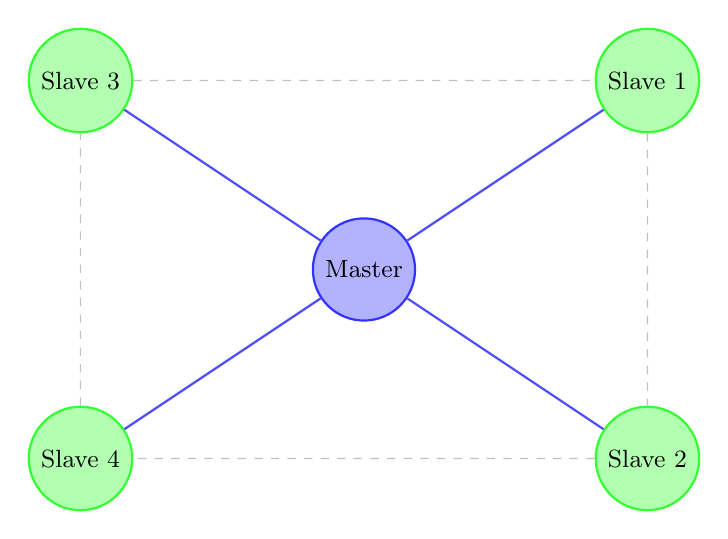
\begin{tikzpicture}[scale=1.2]
  \tikzstyle{master}=[circle, draw=blue!80, fill=blue!30, thick, minimum size=1.2cm, font=\small]
  \tikzstyle{slave}=[circle, draw=green!80, fill=green!30, thick, minimum size=1cm, font=\small]
  \tikzstyle{primary}=[-, thick, blue!70]
  \tikzstyle{secondary}=[-, dashed, gray!50]
  
  % Master en el centro
  \node[master] (m) at (0,0) {Master};
  
  % Slaves alrededor
  \node[slave] (s1) at (3,2) {Slave 1};
  \node[slave] (s2) at (3,-2) {Slave 2};
  \node[slave] (s3) at (-3,2) {Slave 3};
  \node[slave] (s4) at (-3,-2) {Slave 4};
  
  % Conexiones primarias (Master-Slave)
  \draw[primary] (m) -- (s1);
  \draw[primary] (m) -- (s2);
  \draw[primary] (m) -- (s3);
  \draw[primary] (m) -- (s4);
  
  % Conexiones secundarias (Slave-Slave para tolerancia a fallos)
  \draw[secondary] (s1) -- (s2);
  \draw[secondary] (s2) -- (s4);
  \draw[secondary] (s4) -- (s3);
  \draw[secondary] (s3) -- (s1);
\end{tikzpicture}
\caption{Topología Master-Slave: líneas sólidas = comunicación primaria, líneas punteadas = heartbeat y elección}
\label{fig:master-slave-topology}
\end{figure}

\subsubsection{Propiedades de la topología Master-Slave}
Para un clúster con \(N\) Slaves:
\begin{itemize}
  \item \textbf{Latencia de consulta}: \(O(1)\) saltos (Master enruta directamente al Slave apropiado)
  \item \textbf{Escalabilidad}: Lineal con el número de Slaves
  \item \textbf{Tolerancia a fallos}: El sistema continúa operando si falla el Master (elección automática)
  \item \textbf{Consistencia}: Eventual, con replicación configurable (factor por defecto: 2)
\end{itemize}

\textbf{Flujo de consulta típico}:
\begin{enumerate}
  \item Cliente envía consulta al Master
  \item Master calcula embeddings semánticos de la consulta
  \item Master identifica Slaves con contenido semánticamente relevante
  \item Master enruta la consulta a los Slaves seleccionados
  \item Slaves ejecutan búsqueda local y devuelven resultados
  \item Master agrega y ordena resultados finales
\end{enumerate}

\section{Roles y organización funcional}

En el sistema Master-Slave propuesto, los roles están claramente diferenciados para optimizar la coordinación y el procesamiento distribuido. El \textbf{Master} actúa como coordinador central del clúster, mientras que los \textbf{Slaves} son los nodos trabajadores que almacenan datos y procesan consultas.

El \textbf{Master} mantiene el índice semántico global de ubicación de recursos. Cuando recibe una consulta, calcula el embedding semántico y determina qué Slaves contienen información relevante. El Master no almacena documentos directamente sino metadatos sobre qué contenido tiene cada Slave.

Los \textbf{Slaves} son nodos autónomos que integran backend, frontend y base de datos. Cada Slave puede atender usuarios directamente a través de su interfaz web, procesar consultas locales y participar en la replicación de datos. Esta arquitectura permite que los Slaves operen de forma independiente incluso si el Master falla temporalmente.

Un aspecto crítico es la \textbf{elección de líder}: si el Master falla, los Slaves ejecutan el algoritmo Bully para elegir un nuevo Master entre los candidatos elegibles. Esto garantiza la continuidad del servicio sin intervención manual.

\subsection{Diagrama de roles e interacciones}

\begin{figure}[H]
\centering
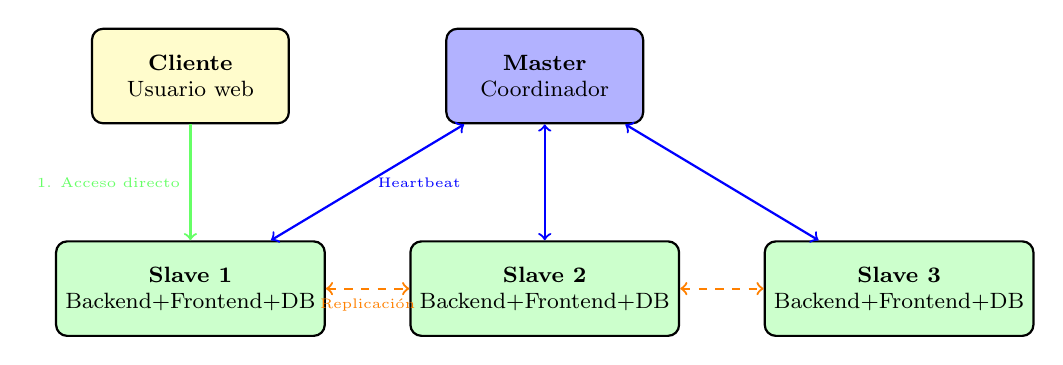
\begin{tikzpicture}[scale=0.9]
  \tikzstyle{role}=[rectangle, draw, thick, minimum width=2.5cm, minimum height=1.2cm, rounded corners, font=\footnotesize, align=center]
  \tikzstyle{master}=[role, fill=blue!30]
  \tikzstyle{slave}=[role, fill=green!20]
  \tikzstyle{client}=[role, fill=yellow!20]
  
  \node[client] (c) at (0,5) {\textbf{Cliente}\\Usuario web};
  \node[master] (m) at (5,5) {\textbf{Master}\\Coordinador};
  \node[slave] (s1) at (0,2) {\textbf{Slave 1}\\Backend+Frontend+DB};
  \node[slave] (s2) at (5,2) {\textbf{Slave 2}\\Backend+Frontend+DB};
  \node[slave] (s3) at (10,2) {\textbf{Slave 3}\\Backend+Frontend+DB};
  
  % Cliente accede a cualquier Slave
  \draw[->, thick, green!60] (c) -- node[left, font=\tiny] {1. Acceso directo} (s1);
  % Master coordina
  \draw[<->, thick, blue] (m) -- node[right, font=\tiny] {Heartbeat} (s1);
  \draw[<->, thick, blue] (m) -- (s2);
  \draw[<->, thick, blue] (m) -- (s3);
  % Replicación entre Slaves
  \draw[<->, thick, orange, dashed] (s1) -- node[below, font=\tiny] {Replicación} (s2);
  \draw[<->, thick, orange, dashed] (s2) -- (s3);
\end{tikzpicture}
\caption{Arquitectura Master-Slave: clientes acceden directamente a Slaves, Master coordina ubicación y replicación}
\label{fig:roles}
\end{figure}

\subsection{Responsabilidades de cada rol}

\begin{table}[H]
\centering
\begin{tabularx}{\textwidth}{|l|X|}
\hline
\textbf{Rol} & \textbf{Responsabilidades} \\ \hline
\textbf{Master} & 
Mantener índice semántico de ubicación de recursos, recibir registros de nuevos documentos, calcular embeddings y determinar relevancia semántica, enrutar consultas a Slaves apropiados, coordinar replicación, monitorear salud del clúster mediante heartbeats, detectar fallos de nodos. \\ \hline
\textbf{Slave} & 
Almacenar documentos en MongoDB local, servir interfaz web (frontend Streamlit), procesar consultas de búsqueda locales, participar en elecciones de líder (algoritmo Bully), enviar heartbeats al Master, recibir y aplicar replicaciones de otros Slaves. \\ \hline
\textbf{Cliente} & 
Acceder a cualquier Slave disponible vía web, realizar búsquedas semánticas y por nombre, subir y descargar documentos, el DNS resuelve distrisearch.local a cualquier Slave saludable. \\ \hline
\end{tabularx}
\caption{Responsabilidades por rol en arquitectura Master-Slave}
\label{tab:responsibilities}
\end{table}

\section{Despliegue y distribución de servicios con Docker}

El despliegue se implementa usando contenedores Docker con una red compartida para el clúster Master-Slave:

\subsection{Arquitectura de redes Docker}

\begin{description}
  \item[cluster-network] Red bridge donde residen el Master, los Slaves y sus bases de datos MongoDB. Permite comunicación directa entre todos los componentes del clúster.
  \item[dns-network] Red opcional para CoreDNS que resuelve \texttt{distrisearch.local} a los Slaves disponibles.
\end{description}

Cada Slave expone sus puertos de backend (8000) y frontend (8501) al host, permitiendo acceso directo desde usuarios externos.

\subsection{Comandos de despliegue}

\textbf{1. Crear red del clúster:}
\begin{verbatim}
docker network create cluster-network
\end{verbatim}

\textbf{2. Desplegar Master:}
\begin{verbatim}
docker run -d --name master --network cluster-network \
  -e NODE_ROLE=master \
  -e NODE_ID=master-001 \
  master-image:latest
\end{verbatim}

\textbf{3. Desplegar Slaves con MongoDB local:}
\begin{verbatim}
docker run -d --name mongo-slave1 --network cluster-network \
  mongo:latest
docker run -d --name slave-001 --network cluster-network \
  -e NODE_ROLE=slave \
  -e NODE_ID=slave-001 \
  -e MASTER_HOST=master \
  -p 8000:8000 -p 8501:8501 \
  slave-image:latest
\end{verbatim}

\begin{figure}[H]
\centering
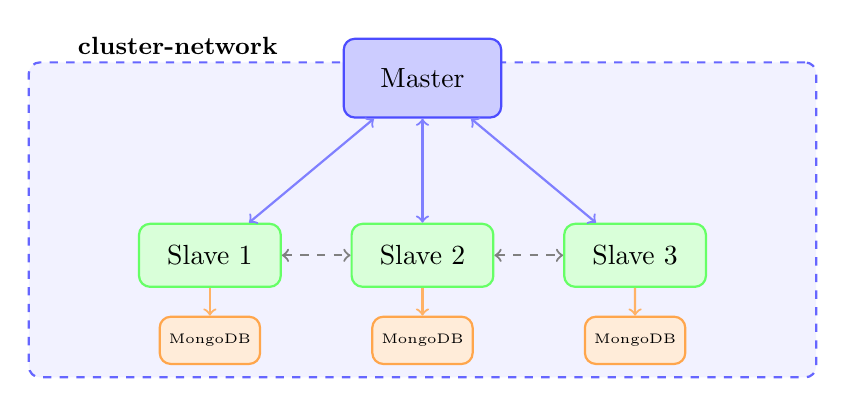
\begin{tikzpicture}[scale=0.9]
  \tikzstyle{net}=[rectangle, draw, thick, dashed, minimum width=10cm, minimum height=4cm, rounded corners]
  \tikzstyle{container}=[rectangle, draw=green!60, fill=green!15, thick, minimum width=1.8cm, minimum height=0.8cm, rounded corners]
  \tikzstyle{master}=[rectangle, draw=blue!70, fill=blue!20, thick, minimum width=2cm, minimum height=1cm, rounded corners]
  \tikzstyle{db}=[rectangle, draw=orange!70, fill=orange!15, thick, minimum width=1.2cm, minimum height=0.6cm, rounded corners]
  
  % Red del clúster
  \node[net, draw=blue!60, fill=blue!5] (cluster) at (3,2) {};
  \node[above right, font=\small] at (-2,4.2) {\textbf{cluster-network}};
  
  % Master
  \node[master] (m) at (3,4) {Master};
  
  % Slaves con MongoDB
  \node[container] (s1) at (0,1.5) {Slave 1};
  \node[db] (db1) at (0,0.3) {\tiny MongoDB};
  \node[container] (s2) at (3,1.5) {Slave 2};
  \node[db] (db2) at (3,0.3) {\tiny MongoDB};
  \node[container] (s3) at (6,1.5) {Slave 3};
  \node[db] (db3) at (6,0.3) {\tiny MongoDB};
  
  % Conexiones Master-Slave
  \draw[<->, thick, blue!50] (m) -- (s1);
  \draw[<->, thick, blue!50] (m) -- (s2);
  \draw[<->, thick, blue!50] (m) -- (s3);
  
  % Conexiones Slave-DB
  \draw[->, thick, orange!60] (s1) -- (db1);
  \draw[->, thick, orange!60] (s2) -- (db2);
  \draw[->, thick, orange!60] (s3) -- (db3);
  
  % Heartbeat entre Slaves
  \draw[<->, thick, dashed, gray] (s1) -- (s2);
  \draw[<->, thick, dashed, gray] (s2) -- (s3);
\end{tikzpicture}
\caption{Clúster Master-Slave: Master coordina, cada Slave tiene MongoDB local, líneas punteadas = heartbeat}
\label{fig:docker-deploy}
\end{figure}

\subsection{Ventajas del diseño}

\begin{itemize}
  \item \textbf{Simplicidad}: Una sola red para todo el clúster
  \item \textbf{Escalabilidad}: Nuevos Slaves se registran automáticamente con el Master
  \item \textbf{Tolerancia a fallos}: Si el Master falla, un Slave es elegido nuevo líder (algoritmo Bully)
  \item \textbf{Acceso directo}: Usuarios acceden a cualquier Slave sin necesidad de gateway
\end{itemize}

\section{Procesos y patrones de diseño}

Cada nodo del clúster ejecuta procesos especializados según su rol. Los \textbf{Slaves} ejecutan: un servidor FastAPI para el backend, un servidor Streamlit para el frontend, un servicio de heartbeat UDP para detección de fallos, y un cliente MongoDB para persistencia local. El \textbf{Master} ejecuta adicionalmente: el índice semántico de ubicación, el balanceador de carga, y el coordinador de replicación.

En términos de concurrencia, el sistema utiliza \texttt{asyncio} de Python para manejar múltiples conexiones y operaciones I/O sin bloqueos. Los heartbeats se procesan en un hilo separado usando UDP para minimizar latencia. El patrón adoptado combina arquitectura dirigida por eventos (event-driven) con paso de mensajes, ideal para sistemas distribuidos donde la latencia de red domina el tiempo de ejecución.

\subsection{Arquitectura interna de un Slave}

\begin{figure}[H]
\centering
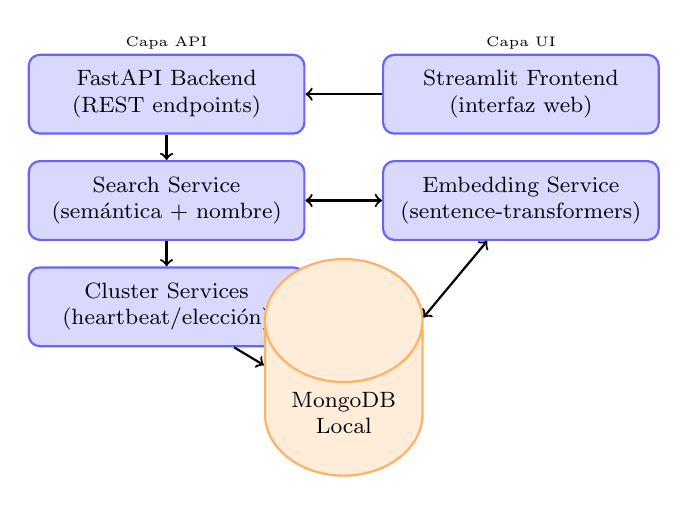
\begin{tikzpicture}[scale=0.9, node distance=1.5cm]
  \tikzstyle{component}=[rectangle, draw=blue!60, fill=blue!15, thick, minimum width=3.5cm, minimum height=1cm, rounded corners, font=\footnotesize, align=center]
  \tikzstyle{storage}=[cylinder, draw=orange!60, fill=orange!15, thick, minimum width=2cm, minimum height=1.2cm, shape border rotate=90, font=\footnotesize, align=center]
  
  % Componentes principales
  \node[component] (api) at (0,4) {FastAPI Backend\\(REST endpoints)};
  \node[component] (search) at (0,2.5) {Search Service\\(semántica + nombre)};
  \node[component] (cluster) at (0,1) {Cluster Services\\(heartbeat/elección)};
  \node[component] (frontend) at (5,4) {Streamlit Frontend\\(interfaz web)};
  \node[component] (embed) at (5,2.5) {Embedding Service\\(sentence-transformers)};
  
  % Almacenamiento
  \node[storage] (mongo) at (2.5,-0.5) {MongoDB\\Local};
  
  % Conexiones
  \draw[->, thick] (api) -- (search);
  \draw[->, thick] (search) -- (cluster);
  \draw[->, thick] (cluster) -- (mongo);
  \draw[<->, thick] (search) -- (embed);
  \draw[->, thick] (frontend) -- (api);
  \draw[<->, thick] (embed) -- (mongo);
  
  % Etiquetas
  \node[above, font=\tiny] at (0,4.5) {Capa API};
  \node[above, font=\tiny] at (5,4.5) {Capa UI};
\end{tikzpicture}
\caption{Arquitectura de un Slave: integra backend, frontend, búsqueda semántica y servicios de clúster}
\label{fig:peer-architecture}
\end{figure}

\subsection{Patrones de diseño aplicados}

\begin{description}
  \item[Event-Driven Architecture] — Cada componente reacciona a eventos (llegada de mensajes, timeouts, cambios de estado)
  \item[Message Passing] — Comunicación entre componentes mediante colas de mensajes asíncronas
  \item[Reactor Pattern] — Event loop que multiplexea I/O de múltiples sockets
  \item[Strategy Pattern] — Algoritmos de routing y replicación intercambiables
  \item[Observer Pattern] — Notificación de cambios de estado de red a componentes interesados
\end{description}

\subsection{Modelo de concurrencia}

\begin{figure}[H]
\centering
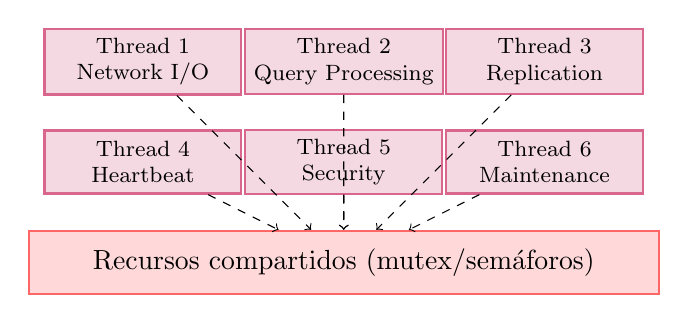
\begin{tikzpicture}[scale=0.85]
  \tikzstyle{thread}=[rectangle, draw=purple!60, fill=purple!15, thick, minimum width=2.5cm, minimum height=0.8cm, font=\footnotesize, align=center]
  
  \node[thread] (t1) at (0,3) {Thread 1\\Network I/O};
  \node[thread] (t2) at (3,3) {Thread 2\\Query Processing};
  \node[thread] (t3) at (6,3) {Thread 3\\Replication};
  \node[thread] (t4) at (0,1.5) {Thread 4\\Heartbeat};
  \node[thread] (t5) at (3,1.5) {Thread 5\\Security};
  \node[thread] (t6) at (6,1.5) {Thread 6\\Maintenance};
  
  % Recursos compartidos
  \node[rectangle, draw=red!60, fill=red!15, thick, minimum width=8cm, minimum height=0.8cm] (shared) at (3,0) {Recursos compartidos (mutex/semáforos)};
  
  \draw[->, dashed] (t1) -- (shared);
  \draw[->, dashed] (t2) -- (shared);
  \draw[->, dashed] (t3) -- (shared);
  \draw[->, dashed] (t4) -- (shared);
  \draw[->, dashed] (t5) -- (shared);
  \draw[->, dashed] (t6) -- (shared);
\end{tikzpicture}
\caption{Modelo de threads para manejo concurrente de operaciones}
\label{fig:concurrency}
\end{figure}

\section{Comunicación entre nodos}

\subsection{Modelo de comunicación por capas}

El sistema implementa una \textbf{arquitectura en capas} para la comunicación que separa las responsabilidades en tres niveles. La \textbf{capa de aplicación} define un protocolo de mensajería de alto nivel con mensajes como \texttt{REGISTER}, \texttt{HEARTBEAT}, \texttt{ELECTION}, \texttt{REPLICATE} y \texttt{QUERY}. Esta capa contiene la lógica de coordinación Master-Slave, ubicación semántica de recursos y gestión de estado del clúster.

La \textbf{capa de transporte} utiliza HTTP/REST (TCP) para operaciones de API como registro de documentos, consultas y replicación. Para heartbeats entre nodos se emplea UDP, optimizado para baja latencia y tolerancia a pérdidas ocasionales. Esta capa también gestiona conexiones persistentes mediante pools de conexiones HTTP.

La \textbf{capa de red} utiliza routing IP estándar sobre la red Docker interna. El dominio \texttt{distrisearch.local} se resuelve mediante CoreDNS a cualquier Slave saludable, proporcionando descubrimiento automático de servicios.

\subsection{Tipos de comunicación}

\subsubsection{Comunicación Master-Slave}
Los Slaves se comunican con el Master mediante REST API para: registrar nuevos documentos (el Master actualiza su índice semántico), recibir instrucciones de replicación, y reportar estado de salud. El Master inicia comunicación con Slaves para: enrutar consultas a nodos relevantes, coordinar replicación, y verificar disponibilidad.

\subsubsection{Comunicación Slave-Slave}
Los Slaves se comunican entre sí para: heartbeats UDP (detección de fallos), mensajes de elección (algoritmo Bully cuando el Master falla), y transferencia directa de réplicas. Esta comunicación no pasa por el Master, garantizando continuidad ante fallos del coordinador.

\subsubsection{Comunicación Cliente-Sistema}
Los usuarios acceden directamente a cualquier Slave mediante su interfaz web Streamlit. El DNS resuelve \texttt{distrisearch.local} a Slaves disponibles, proporcionando balanceo de carga implícito. No existe gateway centralizado; cada Slave es autónomo para atender usuarios.

\subsection{Protocolo de mensajería}
Se definen los siguientes tipos de mensajes:

\begin{table}[H]
\centering
\begin{tabularx}{\textwidth}{|l|X|}
\hline
\textbf{Mensaje} & \textbf{Descripción} \\ \hline
\texttt{REGISTER(doc\_id, embedding)} & Slave notifica al Master sobre nuevo documento con su embedding semántico \\ \hline
\texttt{HEARTBEAT(node\_id, status)} & Slave envía estado de salud al Master y otros Slaves (UDP) \\ \hline
\texttt{ELECTION(node\_id)} & Mensaje del algoritmo Bully: inicio de elección de nuevo Master \\ \hline
\texttt{OK(node\_id)} & Respuesta en elección: nodo con ID mayor responde que tomará el liderazgo \\ \hline
\texttt{COORDINATOR(node\_id)} & Anuncio del nuevo Master elegido a todos los Slaves \\ \hline
\texttt{REPLICATE(doc\_id, data, target)} & Instrucción de replicar documento hacia Slave objetivo \\ \hline
\texttt{QUERY(embedding, top\_k)} & Consulta semántica: Master enruta a Slaves con contenido similar \\ \hline
\end{tabularx}
\caption{Tipos de mensajes del protocolo Master-Slave}
\label{tab:messages}
\end{table}

\subsection{Algoritmo de elección de líder: Bully}
Cuando un Slave detecta que el Master no responde (timeout en heartbeats):

\begin{algorithm}[H]
\caption{Algoritmo Bully para elección de Master}
\begin{algorithmic}[1]
\State \textbf{Input:} nodo actual $P_i$, conjunto de nodos $\{P_1, ..., P_n\}$ ordenados por ID
\State $P_i$ envía mensaje ELECTION a todos $P_j$ donde $j > i$
\If{ningún $P_j$ responde con OK en timeout}
    \State $P_i$ se convierte en Master
    \State $P_i$ envía COORDINATOR a todos los nodos
\Else
    \State $P_i$ espera mensaje COORDINATOR del nodo con mayor ID
\EndIf
\end{algorithmic}
\end{algorithm}

\textbf{Ejemplo}: Si el Master (ID=100) falla y los Slaves tienen IDs 50, 60, 70:
\begin{enumerate}
  \item Slave-50 detecta fallo, envía ELECTION a 60, 70
  \item Slave-60 y 70 responden OK (tienen ID mayor)
  \item Slave-60 envía ELECTION a 70
  \item Slave-70 responde OK
  \item Slave-70 no tiene nadie con ID mayor, se convierte en Master
  \item Slave-70 envía COORDINATOR a todos: nuevo Master elegido
\end{enumerate}

\section{Coordinación y sincronización}

\subsection{Modelo de coordinación}

\subsubsection{Desacoplamiento temporal y referencial}

El sistema implementa diferentes niveles de acoplamiento según el tipo de operación:

\begin{table}[H]
\centering
\begin{tabularx}{\textwidth}{|l|X|X|}
\hline
\textbf{Operación} & \textbf{Acoplamiento temporal} & \textbf{Acoplamiento referencial} \\ \hline
Consulta directa & Acoplado (síncrono) & Acoplado (peer específico) \\ \hline
Replicación & Desacoplado (asíncrono) & Acoplado (réplicas específicas) \\ \hline
Búsqueda flooding & Desacoplado & Parcialmente desacoplado \\ \hline
Heartbeat & Desacoplado & Acoplado (vecinos) \\ \hline
\end{tabularx}
\caption{Niveles de acoplamiento por tipo de operación}
\label{tab:coupling}
\end{table}

El sistema implementa dos modos principales de comunicación con diferentes características de acoplamiento. La \textbf{comunicación directa} es temporalmente acoplada, lo que significa que ambos nodos (emisor y receptor) deben estar activos simultáneamente para completar la interacción. También es referencialmente acoplada porque el emisor conoce explícitamente la identidad del receptor. Este modo se utiliza para consultas síncronas donde se espera una respuesta inmediata y para transferencias de datos que requieren confirmación.

Por otro lado, la \textbf{comunicación basada en eventos} es temporalmente desacoplada, permitiendo que publicación y suscripción ocurran en momentos diferentes sin requerir sincronía estricta. También es referencialmente desacoplada ya que los publicadores no necesitan conocer la identidad de los suscriptores. Este patrón se emplea para notificaciones de cambios de estado, detección de fallos y propagación de eventos que múltiples nodos pueden consumir.

\subsection{Sincronización de acciones}

\subsubsection{Protocolo de sincronización para operaciones distribuidas}

\textbf{Protocolo de timestamps de Lamport:} El sistema utiliza relojes lógicos para establecer un ordenamiento parcial de eventos distribuidos. Cada nodo mantiene un contador $L_i$ que se incrementa en cada evento local. Cuando un nodo envía un mensaje, primero incrementa su reloj ($L_i := L_i + 1$) y adjunta este timestamp al mensaje. Al recibir un mensaje con timestamp $T$, el nodo receptor actualiza su reloj tomando el máximo entre su valor actual y el recibido, luego lo incrementa: $L_i := \max(L_i, T) + 1$. Este mecanismo garantiza que si un evento $a$ causalmente precede a un evento $b$, entonces el timestamp de $a$ será menor que el de $b$. Para resolver empates cuando dos eventos tienen el mismo timestamp, se utiliza el identificador del nodo como criterio de desempate: $(T_1, node_1) < (T_2, node_2)$ si $T_1 < T_2$, o si $T_1 = T_2$ y $node_1 < node_2$.

\subsection{Toma de decisiones distribuidas}

\subsubsection{Consenso para operaciones críticas}

\textbf{Escenario:} Decidir qué nodo se encarga de una tarea (ej: convertirse en coordinador de zona).

\textbf{Algoritmo de elección de líder (simplificado):}
\begin{enumerate}
  \item Cuando se detecta ausencia de coordinador, cada nodo calcula prioridad: \\
  $P_i = h(\text{node\_id}_i, \text{load}_i, \text{uptime}_i)$
  \item Cada nodo anuncia su prioridad a sus vecinos
  \item Nodo con mayor prioridad y confirmación de $\geq 2/3$ vecinos se designa líder
  \item Líder anuncia su rol a toda la red mediante flooding
\end{enumerate}

\textbf{Consenso para cambios de configuración:}
\begin{itemize}
  \item Cambios críticos (ej: modificar factor de replicación) requieren consenso
  \item Se usa votación de mayoría simple o algoritmo Raft simplificado
  \item Solo se aplica cambio si $> 50\%$ de nodos activos aprueban
\end{itemize}

\section{Localización y nombrado de datos / recursos}

Cada documento en el sistema tiene un identificador único (UUID generado al subir) y un \textbf{embedding semántico} de 384 dimensiones que representa su contenido. El mecanismo de localización se basa en \textbf{similitud semántica} en lugar de funciones hash, lo que permite ubicar documentos según su significado y no según propiedades arbitrarias de su identificador.

El Master mantiene un \textbf{índice de ubicación semántica} que mapea cada Slave a un perfil semántico agregado de sus documentos. Cuando llega una consulta, el Master calcula su embedding y determina qué Slaves tienen contenido semánticamente similar.

\subsection{Estrategias de localización de datos}

\subsubsection{Estrategia 1: Búsqueda semántica centralizada}
\begin{algorithm}[H]
\caption{Búsqueda semántica en Master}
\begin{algorithmic}[1]
\State \textbf{Input:} $query$ (texto de consulta), $top\_k$ (número de resultados)
\State \textbf{Output:} lista de documentos relevantes
\State $q\_embedding \gets$ calcular\_embedding($query$)
\State $slaves \gets$ ordenar\_slaves\_por\_similitud($q\_embedding$)
\State $results \gets []$
\For{$slave$ en $slaves[:3]$}  \Comment{Top 3 Slaves más relevantes}
    \State $local\_results \gets$ enviar\_query($slave$, $query$)
    \State $results \gets results \cup local\_results$
\EndFor
\State \Return ordenar\_por\_relevancia($results$)[:$top\_k$]
\end{algorithmic}
\end{algorithm}

\subsubsection{Estrategia 2: Asignación por afinidad semántica}
Asignar cada documento al Slave cuyo perfil semántico es más similar:
$$\text{slave\_destino} = \arg\max_{s \in \text{slaves}} \cos(embedding_{doc}, profile_s)$$
donde $\cos$ es la similitud coseno entre vectores.

\textbf{Ejemplo}: Un documento sobre "algoritmos de ordenamiento" tiene un embedding que el Master compara con los perfiles de cada Slave. Si Slave-2 ya contiene documentos sobre "estructuras de datos" y "complejidad algorítmica", su perfil será semánticamente cercano, por lo que el nuevo documento se almacena allí.

\begin{figure}[H]
\centering
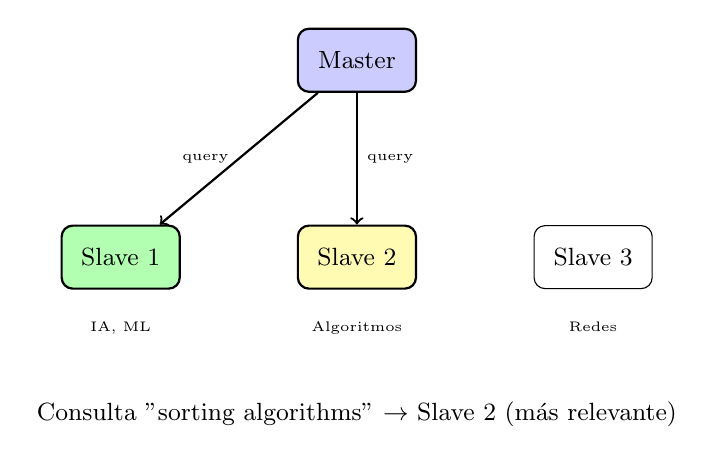
\begin{tikzpicture}[scale=1.0]
  \tikzstyle{node}=[rectangle, draw, minimum width=1.5cm, minimum height=0.8cm, font=\small, rounded corners]
  \tikzstyle{master}=[fill=blue!20, thick]
  \tikzstyle{primary}=[fill=green!30, thick]
  \tikzstyle{replica}=[fill=yellow!30, thick]
  
  % Master
  \node[node, master] (m) at (3,4) {Master};
  
  % Slaves
  \node[node, primary] (s1) at (0,1.5) {Slave 1};
  \node[node, replica] (s2) at (3,1.5) {Slave 2};
  \node[node] (s3) at (6,1.5) {Slave 3};
  
  % Perfiles semánticos
  \node[font=\tiny, below] at (0,0.8) {IA, ML};
  \node[font=\tiny, below] at (3,0.8) {Algoritmos};
  \node[font=\tiny, below] at (6,0.8) {Redes};
  
  % Conexiones
  \draw[->, thick] (m) -- node[left, font=\tiny] {query} (s1);
  \draw[->, thick] (m) -- node[right, font=\tiny] {query} (s2);
  
  % Leyenda
  \node[font=\small] at (3,-0.5) {Consulta "sorting algorithms" $\rightarrow$ Slave 2 (más relevante)};
\end{tikzpicture}
\caption{Ubicación semántica: Master enruta consultas a Slaves con contenido similar}
\label{fig:data-location}
\end{figure}

\section{Distribución, replicación y consistencia de datos}

El sistema implementa replicación de datos donde cada documento puede tener $k$ réplicas en diferentes Slaves (por defecto $k = 2$) para garantizar tolerancia a fallos y alta disponibilidad. El coordinador de replicación en el Master selecciona Slaves con \textbf{afinidad semántica}: documentos similares se replican en Slaves que ya contienen contenido relacionado, mejorando la localidad de las consultas.

Respecto a la consistencia, los documentos son inmutables una vez subidos, simplificando el modelo al eliminar la necesidad de sincronizar actualizaciones.

\subsection{Estrategia de replicación}
Para un factor de replicación $k=2$, al almacenar un documento en el Slave primario $S_p$, el Master selecciona $k-1 = 1$ Slaves adicionales para réplicas. Los criterios de selección son:
\begin{itemize}
  \item \textbf{Afinidad semántica}: Preferir Slaves cuyo perfil sea similar al embedding del documento
  \item \textbf{Carga actual}: Balancear distribución de almacenamiento entre Slaves
  \item \textbf{Disponibilidad}: Priorizar Slaves con historial de uptime alto
\end{itemize}

\begin{figure}[H]
\centering
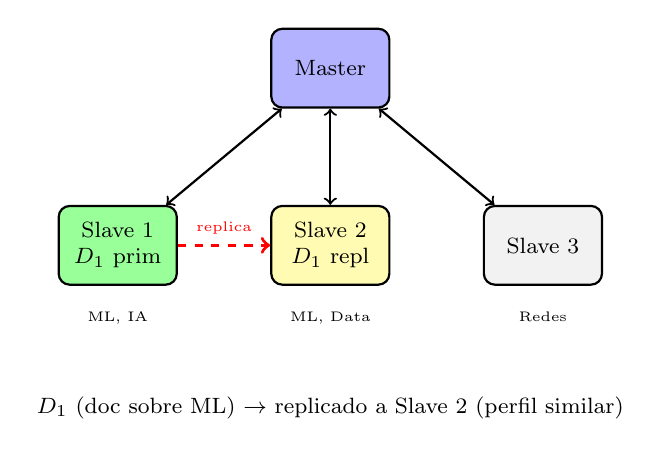
\begin{tikzpicture}[scale=0.9]
  \tikzstyle{node}=[rectangle, draw, thick, minimum width=1.5cm, minimum height=1cm, font=\footnotesize, align=center, rounded corners]
  \tikzstyle{master}=[fill=blue!30]
  \tikzstyle{primary}=[fill=green!40]
  \tikzstyle{replica}=[fill=yellow!30]
  \tikzstyle{normal}=[fill=gray!10]
  
  % Master
  \node[node, master] (m) at (3,4) {Master};
  
  % Slaves
  \node[node, primary] (s1) at (0,1.5) {Slave 1\\$D_1$ prim};
  \node[node, replica] (s2) at (3,1.5) {Slave 2\\$D_1$ repl};
  \node[node, normal] (s3) at (6,1.5) {Slave 3};
  
  % Perfiles
  \node[font=\tiny, below] at (0,0.7) {ML, IA};
  \node[font=\tiny, below] at (3,0.7) {ML, Data};
  \node[font=\tiny, below] at (6,0.7) {Redes};
  
  % Conexiones
  \draw[<->, thick] (m) -- (s1);
  \draw[<->, thick] (m) -- (s2);
  \draw[<->, thick] (m) -- (s3);
  
  % Flecha de replicación
  \draw[->, very thick, red, dashed] (s1) -- node[midway, above] {\tiny replica} (s2);
  
  % Leyenda
  \node[font=\footnotesize, below] at (3,-0.5) {$D_1$ (doc sobre ML) $\rightarrow$ replicado a Slave 2 (perfil similar)};
\end{tikzpicture}
\caption{Replicación por afinidad semántica: documento ML replicado a Slave con perfil similar}
\label{fig:replication}
\end{figure}

\subsection{Modelo de consistencia}

El sistema adopta un modelo de \textbf{consistencia eventual} con las siguientes características:
\begin{itemize}
  \item \textbf{Escrituras}: Documentos nuevos se escriben primero en el Slave que recibe la subida, luego se replican
  \item \textbf{Lecturas}: Cualquier Slave con una réplica puede responder consultas
  \item \textbf{Convergencia}: Garantizada por la naturaleza inmutable de los documentos
\end{itemize}

\section{Tolerancia a fallos, robustez y dinámicas de red}

El sistema proporciona soporte integral para fallos parciales, incluyendo: Slaves que se desconectan temporalmente, fallo del Master (recuperado mediante elección Bully), y reincorporación de nodos nuevos o recuperados.

La arquitectura Master-Slave con elección de líder garantiza continuidad: si el Master falla, los Slaves detectan la ausencia de heartbeats y ejecutan el algoritmo Bully para elegir un nuevo coordinador.

Cuando un Slave nuevo se une a la red o un Slave existente falla:
\begin{itemize}
  \item \textbf{Nuevo Slave}: Se registra con el Master enviando su perfil semántico inicial
  \item \textbf{Fallo de Slave}: El Master detecta ausencia de heartbeats y marca el nodo como no disponible
  \item \textbf{Fallo de Master}: Slaves detectan timeout, inician elección Bully, nuevo Master asume coordinación
  \item \textbf{Rerreplicación}: Si un Slave con réplicas falla, el Master coordina crear nuevas réplicas en otros Slaves
\end{itemize}

\subsection{Detección de fallos mediante Heartbeat}
\begin{algorithm}[H]
\caption{Protocolo Heartbeat para detección de fallos}
\begin{algorithmic}[1]
\State \textbf{Constantes:} $T_{heartbeat} = 5s$, $T_{timeout} = 15s$
\While{nodo está activo}
    \For{cada vecino $v$ en lista de vecinos}
        \State Enviar \texttt{PING} a $v$
        \If{no se recibe \texttt{PONG} en $T_{timeout}$}
            \State Marcar $v$ como fallido
            \State Notificar a otros vecinos sobre fallo de $v$
            \State Intentar reconexión o buscar reemplazo
        \EndIf
    \EndFor
    \State Esperar $T_{heartbeat}$
\EndWhile
\end{algorithmic}
\end{algorithm}

\subsection{Protocolo de incorporación de nuevo nodo (JOIN)}
\begin{figure}[H]
\centering
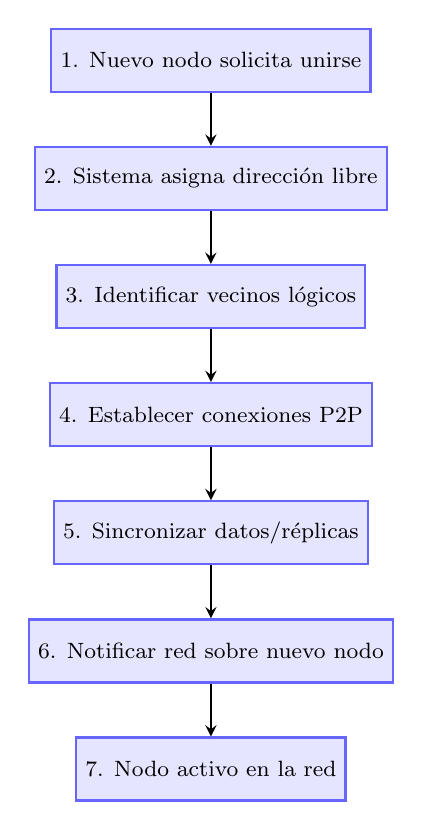
\begin{tikzpicture}[scale=0.8, node distance=1.5cm]
  \tikzstyle{process}=[rectangle, draw=blue!60, fill=blue!10, thick, minimum width=3cm, minimum height=0.8cm, font=\footnotesize, align=center]
  \tikzstyle{arrow}=[->, thick, >=stealth]
  
  \node[process] (s1) {1. Nuevo nodo solicita unirse};
  \node[process, below of=s1] (s2) {2. Sistema asigna dirección libre};
  \node[process, below of=s2] (s3) {3. Identificar vecinos lógicos};
  \node[process, below of=s3] (s4) {4. Establecer conexiones P2P};
  \node[process, below of=s4] (s5) {5. Sincronizar datos/réplicas};
  \node[process, below of=s5] (s6) {6. Notificar red sobre nuevo nodo};
  \node[process, below of=s6] (s7) {7. Nodo activo en la red};
  
  \draw[arrow] (s1) -- (s2);
  \draw[arrow] (s2) -- (s3);
  \draw[arrow] (s3) -- (s4);
  \draw[arrow] (s4) -- (s5);
  \draw[arrow] (s5) -- (s6);
  \draw[arrow] (s6) -- (s7);
\end{tikzpicture}
\caption{Proceso de incorporación de nuevo nodo a la red P2P}
\label{fig:join-protocol}
\end{figure}

\subsection{Manejo de fallo de nodo}
Cuando un nodo $N$ falla:

\begin{enumerate}
  \item \textbf{Detección}: Vecinos detectan fallo por timeout de heartbeat
  \item \textbf{Notificación}: Vecinos notifican al resto de la red
  \item \textbf{Reconexión}: Vecinos de $N$ se conectan entre sí para mantener conectividad
  \item \textbf{Re-replicación}: Datos con réplicas en $N$ se replican en otros nodos
  \item \textbf{Actualización de rutas}: Tablas de routing se actualizan
\end{enumerate}

\begin{figure}[H]
\centering
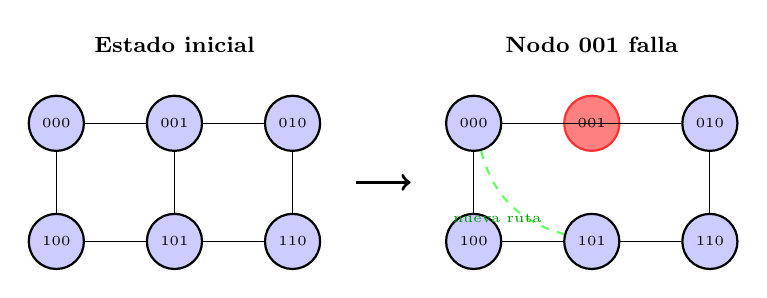
\begin{tikzpicture}[scale=1.0]
  % Estado inicial
  \begin{scope}
    \node[font=\footnotesize\bfseries] at (1.5,2.5) {Estado inicial};
    \tikzstyle{node}=[circle, draw, thick, minimum size=0.7cm, font=\tiny, fill=blue!20]
    \tikzstyle{failed}=[fill=red!50]
    
    \node[node] (a1) at (0,1.5) {000};
    \node[node] (b1) at (1.5,1.5) {001};
    \node[node] (c1) at (3,1.5) {010};
    \node[node] (d1) at (0,0) {100};
    \node[node] (e1) at (1.5,0) {101};
    \node[node] (f1) at (3,0) {110};
    
    \draw[-] (a1) -- (b1);
    \draw[-] (b1) -- (c1);
    \draw[-] (a1) -- (d1);
    \draw[-] (b1) -- (e1);
    \draw[-] (c1) -- (f1);
    \draw[-] (d1) -- (e1);
    \draw[-] (e1) -- (f1);
  \end{scope}
  
  % Flecha de transición
  \draw[->, very thick] (3.8,0.75) -- (4.5,0.75);
  
  % Estado después del fallo
  \begin{scope}[xshift=5.3cm]
    \node[font=\footnotesize\bfseries] at (1.5,2.5) {Nodo 001 falla};
    \tikzstyle{node}=[circle, draw, thick, minimum size=0.7cm, font=\tiny, fill=blue!20]
    \tikzstyle{failed}=[fill=red!50, draw=red!80]
    
    \node[node] (a2) at (0,1.5) {000};
    \node[node, failed] (b2) at (1.5,1.5) {001};
    \node[node] (c2) at (3,1.5) {010};
    \node[node] (d2) at (0,0) {100};
    \node[node] (e2) at (1.5,0) {101};
    \node[node] (f2) at (3,0) {110};
    
    \draw[-] (a2) -- (c2);
    \draw[-] (a2) -- (d2);
    \draw[-] (c2) -- (f2);
    \draw[-] (d2) -- (e2);
    \draw[-] (e2) -- (f2);
    \draw[-, dashed, thick, green!60] (a2) to[bend right=30] (e2);
    
    \node[font=\tiny, green!60!black] at (0.3,0.3) {nueva ruta};
  \end{scope}
\end{tikzpicture}
\caption{Reconfiguración de red tras fallo de nodo 001: rutas alternativas y reconexiones}
\label{fig:fault-tolerance}
\end{figure}

\subsection{Métricas de resiliencia}

Para un clúster con $N$ Slaves, el sistema presenta características de resiliencia cuantificables:
\begin{itemize}
  \item \textbf{Tolerancia a fallos de Slaves}: El sistema permanece operativo mientras al menos un Slave esté activo
  \item \textbf{Tolerancia a fallo de Master}: El algoritmo Bully elige nuevo Master en $O(N)$ mensajes
  \item \textbf{Tiempo de detección de fallo}: Determinado por $T_{timeout} = 15s$ (3 heartbeats perdidos)
  \item \textbf{Tiempo de recuperación}: Elección Bully completa en $< 30s$ típicamente
\end{itemize}

\section{Seguridad, autenticación y autorización}

El sistema implementa múltiples capas de seguridad para proteger tanto los datos como la integridad de la red. Cada nodo posee una identidad única basada en criptografía de clave pública (par de claves pública/privada), lo que permite autenticación mutua entre peers antes de establecer comunicación. Toda la comunicación entre nodos se realiza mediante canales cifrados usando TLS (Transport Layer Security), protegiendo los datos en tránsito contra escuchas y manipulación.

El sistema implementa control de acceso mediante permisos que definen qué nodos pueden leer o escribir ciertos datos. Esto se logra usando firmas digitales para verificar autoriz ación, listas de control de acceso (ACLs) basadas en identidad de nodo, y certificados digitales que vinculan identidades con permisos específicos. Para mitigar la presencia de nodos maliciosos, el sistema emplea múltiples mecanismos: verificación de integridad mediante hashes criptográficos (SHA-256) y firmas digitales, sistemas de reputación que rastrean el comportamiento histórico de los nodos, validación de datos mediante consenso entre múltiples peers, limitación de privilegios siguiendo el principio de mínimo privilegio, y protección contra ataques Sybil mediante pruebas de identidad y restricción de nuevas incorporaciones.

\subsection{Modelo de seguridad por capas}

\begin{figure}[H]
\centering
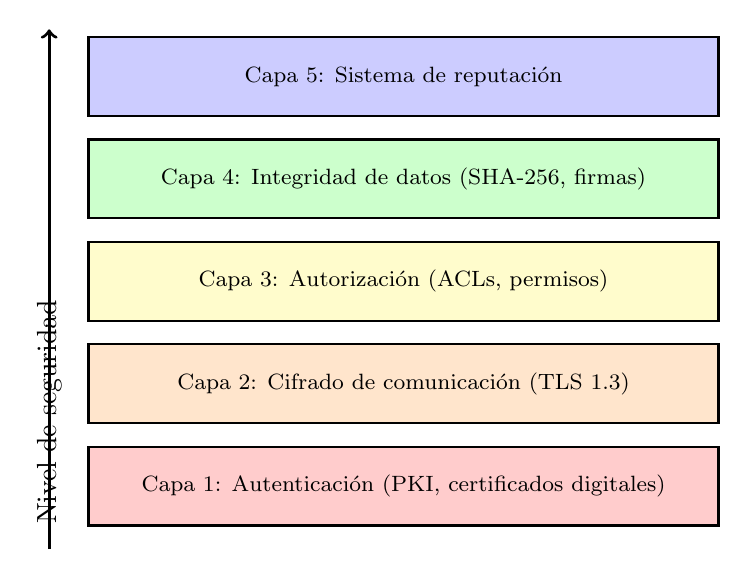
\begin{tikzpicture}[scale=1.0]
  \tikzstyle{layer}=[rectangle, draw, thick, minimum width=8cm, minimum height=1cm, font=\footnotesize]
  
  \node[layer, fill=red!20] (l1) at (0,0) {Capa 1: Autenticación (PKI, certificados digitales)};
  \node[layer, fill=orange!20] (l2) at (0,1.3) {Capa 2: Cifrado de comunicación (TLS 1.3)};
  \node[layer, fill=yellow!20] (l3) at (0,2.6) {Capa 3: Autorización (ACLs, permisos)};
  \node[layer, fill=green!20] (l4) at (0,3.9) {Capa 4: Integridad de datos (SHA-256, firmas)};
  \node[layer, fill=blue!20] (l5) at (0,5.2) {Capa 5: Sistema de reputación};
  
  \draw[->, very thick] (-4.5,-0.8) -- (-4.5,5.8) node[midway, left, rotate=90] {Nivel de seguridad};
\end{tikzpicture}
\caption{Arquitectura de seguridad por capas}
\label{fig:security-layers}
\end{figure}

\subsection{Protocolo de autenticación}

\begin{algorithm}[H]
\caption{Autenticación mutua entre peers}
\begin{algorithmic}[1]
\State \textbf{Nodo A quiere conectarse con Nodo B}
\State A genera nonce $N_A$ aleatorio
\State A $\rightarrow$ B: \texttt{HELLO}($ID_A$, $N_A$, $Cert_A$)
\State B verifica $Cert_A$ con autoridad certificadora
\If{$Cert_A$ es válido}
    \State B genera nonce $N_B$
    \State B $\rightarrow$ A: \texttt{CHALLENGE}($N_B$, $Sign_B(N_A)$, $Cert_B$)
    \State A verifica $Cert_B$ y $Sign_B(N_A)$
    \If{verificación exitosa}
        \State A $\rightarrow$ B: \texttt{RESPONSE}($Sign_A(N_B)$)
        \State B verifica $Sign_A(N_B)$
        \State \textbf{Conexión autenticada establecida}
        \State Establecer canal TLS con claves de sesión
    \EndIf
\EndIf
\end{algorithmic}
\end{algorithm}

\subsection{Control de acceso basado en permisos}

Cada dato tiene asociado un descriptor de seguridad:

\begin{table}[H]
\centering
\begin{tabularx}{0.9\textwidth}{|l|X|}
\hline
\textbf{Campo} & \textbf{Descripción} \\ \hline
\texttt{owner} & ID del nodo propietario del dato \\ \hline
\texttt{readers} & Lista de nodos con permiso de lectura \\ \hline
\texttt{writers} & Lista de nodos con permiso de escritura \\ \hline
\texttt{signature} & Firma digital del propietario \\ \hline
\texttt{hash} & Hash SHA-256 para verificar integridad \\ \hline
\texttt{timestamp} & Marca temporal de creación/modificación \\ \hline
\end{tabularx}
\caption{Descriptor de seguridad de datos}
\label{tab:security-descriptor}
\end{table}

\subsection{Sistema de reputación contra nodos maliciosos}

Cada nodo mantiene una tabla de reputación de sus vecinos que se actualiza continuamente según un modelo de promedio ponderado exponencial: $R_i(t+1) = \alpha \cdot R_i(t) + (1-\alpha) \cdot B_i(t)$, donde $R_i(t)$ representa la reputación del nodo $i$ en el tiempo $t$, $B_i(t)$ captura el comportamiento reciente tomando valor $1$ para comportamiento bueno y $0$ para comportamiento malo, y $\alpha = 0.9$ es el factor de decaimiento que da mayor peso al historial. 

El sistema toma acciones diferenciadas según el nivel de reputación: nodos con $R_i > 0.8$ son considerados confiables y reciben prioridad alta en routing y almacenamiento; nodos con $0.5 < R_i \leq 0.8$ son tratados como normales sin privilegios especiales ni restricciones; nodos con $0.3 < R_i \leq 0.5$ son clasificados como sospechosos y sometidos a monitoreo aumentado; finalmente, nodos con $R_i \leq 0.3$ son bloqueados y desconectados de la red para proteger la integridad del sistema.

\subsection{Mitigación de ataques comunes}

\begin{table}[H]
\centering
\begin{tabularx}{\textwidth}{|l|X|X|}
\hline
\textbf{Ataque} & \textbf{Descripción} & \textbf{Mitigación} \\ \hline
Sybil & Crear múltiples identidades falsas & PKI + verificación de identidad + límite de nodos por IP \\ \hline
Eclipse & Aislar nodo víctima & Diversificación de conexiones + monitoreo de conectividad \\ \hline
Man-in-the-Middle & Interceptar comunicaciones & TLS 1.3 + autenticación mutua \\ \hline
Data poisoning & Insertar datos corruptos & Firmas digitales + verificación de hash + reputación \\ \hline
DDoS & Saturar nodos con peticiones & Rate limiting + listas negras + sistema de reputación \\ \hline
\end{tabularx}
\caption{Ataques comunes y mecanismos de mitigación}
\label{tab:attacks}
\end{table}

\section{Análisis de Calidad del Sistema}

\subsection{Propiedades del diseño}

El sistema presenta 4 propiedades fundamentales que caracterizan su arquitectura. La \textbf{descentralización} garantiza que no existe un punto central de fallo, ya que todos los nodos poseen capacidades equivalentes y pueden asumir cualquier rol necesario. La \textbf{redundancia} se manifiesta en múltiples rutas alternativas entre nodos y en la replicación de datos a través de múltiples nodos. La \textbf{escalabilidad} se logra mediante un crecimiento logarítmico tanto de los recursos requeridos por nodo como del diámetro de la red respecto al número total de nodos. La \textbf{flexibilidad} permite la incorporación y salida dinámica de nodos sin interrumpir el servicio. 

\subsection{Escalabilidad del diseño}

\begin{table}[H]
\centering
\begin{tabularx}{\textwidth}{|c|c|c|X|}
\hline
\textbf{Slaves} & \textbf{Capacidad} & \textbf{Throughput} & \textbf{Escenario de uso} \\ \hline
3 & 3 TB & 100 qps & Prototipo/Testing \\ \hline
5 & 5 TB & 200 qps & Desarrollo \\ \hline
10 & 10 TB & 500 qps & Producción pequeña \\ \hline
20 & 20 TB & 1000 qps & Producción media \\ \hline
50 & 50 TB & 2500 qps & Producción grande \\ \hline
100 & 100 TB & 5000 qps & Escala empresarial \\ \hline
\end{tabularx}
\caption{Escalabilidad del sistema Master-Slave según número de Slaves}
\label{tab:scalability}
\end{table}

\textbf{Análisis}: La arquitectura Master-Slave presenta escalabilidad lineal con el número de Slaves. Cada Slave agregado aumenta proporcionalmente la capacidad de almacenamiento y el throughput del sistema. El Master se convierte en potencial cuello de botella solo cuando el número de Slaves supera varios cientos, momento en que se pueden implementar técnicas de sharding del índice semántico o replicación del Master. Para la mayoría de casos de uso (hasta 100 Slaves), un solo Master es suficiente.

\subsection{Métricas de rendimiento esperadas}

\begin{table}[H]
\centering
\begin{tabularx}{\textwidth}{|l|X|c|}
\hline
\textbf{Métrica} & \textbf{Descripción} & \textbf{Objetivo} \\ \hline
Disponibilidad & Porcentaje de tiempo que el sistema está operativo & $> 99.5\%$ \\ \hline
Latencia de búsqueda & Tiempo promedio para localizar un dato & $< 500$ms \\ \hline
Tasa de éxito & Porcentaje de búsquedas exitosas & $> 95\%$ \\ \hline
Throughput & Consultas por segundo soportadas & $> 1000$ qps \\ \hline
Overhead de red & Mensajes adicionales vs óptimo teórico & $< 3x$ \\ \hline
MTTR & Tiempo promedio de recuperación tras fallo & $< 30$s \\ \hline
\end{tabularx}
\caption{Métricas de rendimiento del sistema}
\label{tab:performance-metrics}
\end{table}





\section{Conclusión}

Este documento ha presentado la especificación arquitectónica completa de un sistema distribuido Master-Slave con ubicación de recursos por vectorización semántica. El diseño prioriza cinco aspectos fundamentales:

\textbf{Coordinación centralizada con tolerancia a fallos}: El Master coordina el clúster manteniendo el índice semántico de ubicación y el balanceo de carga. Si el Master falla, el algoritmo Bully garantiza elección automática de un nuevo líder entre los Slaves candidatos, eliminando puntos únicos de fallo permanentes.

\textbf{Ubicación semántica de recursos}: En lugar de funciones hash (DHT), el sistema utiliza embeddings de 384 dimensiones generados por sentence-transformers para representar documentos. Esto permite localización basada en similitud de contenido, mejorando la relevancia de búsquedas y la localidad de datos relacionados.

\textbf{Alta disponibilidad}: Cada Slave es autónomo con su propio backend, frontend y base de datos MongoDB. Los usuarios pueden acceder a cualquier Slave directamente, y la replicación por afinidad semántica garantiza que los datos sobrevivan fallos individuales.

\textbf{Escalabilidad horizontal}: Agregar Slaves es trivial: el nuevo nodo se registra con el Master, reporta su perfil semántico, y comienza a recibir consultas y datos. El Master actualiza dinámicamente su índice de ubicación.

\textbf{Simplicidad operativa}: La arquitectura Master-Slave es conceptualmente más simple que topologías P2P complejas como hipercubo, facilitando debugging, monitoreo y mantenimiento del sistema en producción.

\section*{Referencias}
\begin{itemize}
  \item Sentence-Transformers: documentación oficial para generación de embeddings semánticos.
  \item Algoritmo Bully: Garcia-Molina, H. ``Elections in a Distributed Computing System'' (1982).
  \item CoreDNS: documentación oficial para resolución DNS en entornos containerizados.
  \item FastAPI y Streamlit: frameworks utilizados para backend y frontend respectivamente.
\end{itemize}

\end{document}
